%% 
%% Copyright 2007-2025 Elsevier Ltd
%% 
%% This file is part of the 'Elsarticle Bundle'.
%% ---------------------------------------------
%% 
%% It may be distributed under the conditions of the LaTeX Project Public
%% License, either version 1.3 of this license or (at your option) any
%% later version.  The latest version of this license is in
%%    http://www.latex-project.org/lppl.txt
%% and version 1.3 or later is part of all distributions of LaTeX
%% version 1999/12/01 or later.
%% 
%% The list of all files belonging to the 'Elsarticle Bundle' is
%% given in the file `manifest.txt'.
%% 
%% Template article for Elsevier's document class `elsarticle'
%% with numbered style bibliographic references
%% SP 2008/03/01
%% $Id: elsarticle-template-num.tex 272 2025-01-09 17:36:26Z rishi $
%%
% \documentclass[preprint,12pt]{elsarticle}

%% Use the option review to obtain double line spacing
% \documentclass[preprint,review,12pt,times,3p]{elsarticle}

\documentclass[times, review, 10pt]{elsarticle}

\usepackage[T1]{fontenc}
\usepackage[utf8]{inputenc}
\usepackage{lmodern} % 轻量且兼容性好的字体
\usepackage{amsmath,amssymb} % 数学符号
\usepackage{graphicx}
\usepackage{booktabs}
%% Use the options 1p,twocolumn; 3p; 3p,twocolumn; 5p; or 5p,twocolumn
%% for a journal layout:
% \documentclass[final,1p,times]{elsarticle}
%% \documentclass[final,1p,times,twocolumn]{elsarticle}
%% \documentclass[final,3p,times]{elsarticle}
%% \documentclass[final,3p,times,twocolumn]{elsarticle}
%% \documentclass[final,5p,times]{elsarticle}
%% \documentclass[final,5p,times,twocolumn]{elsarticle}

%% For including figures, graphicx.sty has been loaded in
%% elsarticle.cls. If you prefer to use the old commands
%% please give \usepackage{epsfig}

%% The amssymb package provides various useful mathematical symbols
\usepackage{amssymb}
%% The amsmath package provides various useful equation environments.
\usepackage{amsmath}
%% The amsthm package provides extended theorem environments
%% \usepackage{amsthm}

%% The lineno packages adds line numbers. Start line numbering with
%% \begin{linenumbers}, end it with \end{linenumbers}. Or switch it on
%% for the whole article with \linenumbers.
%% \usepackage{lineno}
\usepackage{algorithm}      % 提供 algorithm 浮动体环境
\usepackage{algpseudocode}  % 提供 algorithmic 环境,用于编写伪代码
\usepackage{graphicx}
\usepackage[colorlinks=true, allcolors=blue]{hyperref}
\usepackage[font=small, labelfont=bf]{caption}

\usepackage{rotating} % 必须:用于横向表格
\usepackage{booktabs} % 强烈推荐:用于专业表格线
\usepackage{array}
\usepackage{bbm}

\journal{Pattern Recognition}

\begin{document}

\begin{frontmatter}

%% Title, authors and addresses

%% use the tnoteref command within \title for footnotes;
%% use the tnotetext command for theassociated footnote;
%% use the fnref command within \author or \affiliation for footnotes;
%% use the fntext command for theassociated footnote;
%% use the corref command within \author for corresponding author footnotes;
%% use the cortext command for theassociated footnote;
%% use the ead command for the email address,
%% and the form \ead[url] for the home page:
%% \title{Title\tnoteref{label1}}
%% \tnotetext[label1]{}
%% \author{Name\corref{cor1}\fnref{label2}}
%% \ead{email address}
%% \ead[url]{home page}
%% \fntext[label2]{}
%% \cortext[cor1]{}
%% \affiliation{organization={},
%%             addressline={},
%%             city={},
%%             postcode={},
%%             state={},
%%             country={}}
%% \fntext[label3]{}

\title{Hyper-HierUDA:Hyperbolic Hierarchical Learning for Unsupervised Domain Adaptation in Semantic Segmentation} %% Article title

%% use optional labels to link authors explicitly to addresses:
%% \author[label1,label2]{}
%% \affiliation[label1]{organization={},
%%             addressline={},
%%             city={},
%%             postcode={},
%%             state={},
%%             country={}}
%%
%% \affiliation[label2]{organization={},
%%             addressline={},
%%             city={},
%%             postcode={},
%%             state={},
%%             country={}}

% \author[alabel1]{Xiaokang Zhou} %% Author name

% %% Author affiliation
% \affiliation[alabel1]{
%             organization={Sichuan University},%Department and Organization
%             addressline={No. 24 South Section 1, Yihuan Road}, 
%             city={Chengdu},
%             postcode={610065}, 
%             state={Sichuan Province},
%             country={China}}

% \author[alabel2]{Hua Yan\corref{cor1}}
% \ead{hua.yan@scu.edu.cn}
% \ead[url]{https://eeis.scu.edu.cn/info/1234/xxxx.htm}
% \affiliation[alabel2]{
%             organization={College of Electronic and Information Engineering, Sichuan University},%Department and Organization
%             addressline={No. 24 South Section 1, Yihuan Road}, 
%             city={Chengdu},
%             postcode={610065}, 
%             state={Sichuan Province},
%             country={China}}
% \cortext[cor1]{Corresponding author.}


%% Abstract
\begin{abstract}
Unsupervised Domain Adaptation (UDA) is a key technique for addressing the performance degradation of semantic segmentation models when applied across domains, such as transferring from synthetic to real-world data. Although substantial progress has been made with existing adversarial training and self-training methods, these approaches typically adhere to a “flat” classification paradigm, neglecting the inherent semantic hierarchy among categories. In this work, we propose Hyper-HierUDA, a novel UDA domain generalization strategy that integrates hyperbolic geometry with UDA tasks, significantly enhancing domain generalization by explicitly learning high-level semantic knowledge within hierarchical structures.
Specifically, we conduct UDA in hyperbolic space, leveraging its hierarchical properties to move beyond the conventional flat classification paradigm. This enables a progressive classification approach that incorporates richer high-level semantic knowledge for cross-domain generalization. Furthermore, we introduce an explicit learning strategy for high-level concepts within the hierarchy. Building on the progressive classification paradigm, Hyper-HierUDA requires the model to predict not only specific categories but also their corresponding abstract concepts, utilizing these abstract concepts to strengthen the cross-domain generalization of specific category knowledge.
Experimental results on the GTA5→Cityscapes and Synthia→Cityscapes benchmarks demonstrate that Hyper-HierUDA achieves state-of-the-art performance and is effective across multiple backbone networks, including DAFormer and DeepLabv3+. Notably, our approach yields significant improvements in small-scale and semantically similar categories, such as ``Sidewalk'' and ``Traffic sign''. Extensive ablation studies and feature analyses further validate that explicit learning within hyperbolic hierarchies produces more discriminative and domain-invariant features, thereby efficiently facilitating cross-domain knowledge transfer.
\end{abstract}

%%Graphical abstract


%% Keywords
\begin{keyword}
%% keywords here, in the form: keyword \sep keyword
Unsupervised Domain Adaptation \sep Semantic Segmentation \sep Hyperbolic Geometry \sep Progressive Classification \sep Explicit Semantic Learning

\end{keyword}

\end{frontmatter}

%% Add \usepackage{lineno} before \begin{document} and uncomment 
%% following line to enable line numbers
%% \linenumbers

%% main text
%%

%% Use \section commands to start a section
\section{Introduction}
%% Labels are used to cross-reference an item using \ref command.

Semantic segmentation is a fundamental task in computer vision with broad applications in domains such as autonomous driving and medical image analysis. Although deep learning-based models have achieved remarkable success in this task, their performance is heavily reliant on large amounts of pixel-level annotated data, the acquisition of which is both costly and time-consuming. Leveraging synthetic data—such as the GTAV\cite{richter2016playing} dataset rendered by game engines—as automatically labeled source domain offers an effective solution to this problem. However, due to significant domain shift between synthetic and real-world data, models trained on the source domain exhibit substantial performance degradation\cite{lecun2002gradient} when applied to the target domain. UDA aims to address this issue by adapting a model trained on a labeled source domain to an unlabeled target domain.

Mainstream UDA approaches can be broadly categorized into adversarial methods and self-training methods. Adversarial methods\cite{ganin2015unsupervised} minimize the discrepancy between source and target domains via domain discriminators, but are often hampered by unstable training dynamics\cite{goodfellow2014generative}. Self-training methods iteratively train models using pseudo-labels generated for high-confidence target domain samples, though their performance is limited by the noise inherent\cite{zou2018unsupervised} in the pseudo-labels. Despite notable progress, these methods share a common limitation: they adopt a ``flat'' classification paradigm, mapping each extracted feature directly to one of several mutually independent class labels. As shown in Fig. \ref{fig:flat}, this paradigm overlooks the inherent semantic hierarchy among real-world classes (e.g., both ``Car'' and ``Bus'' are subcategories of ``Vehicle''), thus failing to exploit the powerful prior knowledge for improved domain generalization.

\begin{figure}[htbp] % [htbp] 是位置参数,用于控制图片放置的位置
    \centering          % 让图片居中
    \includegraphics[width=0.5\textwidth]{figure1.png} % 插入图片
    \caption{Flat classification and progressive classification.} % 添加标题
    \label{fig:flat} % 添加标签,用于文中引用
\end{figure}

Meanwhile, hyperbolic geometry has recently attracted attention in deep learning due to its unique properties. Compared to Euclidean space, hyperbolic space possesses exponential expansion capacity, allowing for low-distortion embeddings of tree-like or hierarchically structured data, where parent nodes are located near the center and child nodes are distributed towards the periphery\cite{ganea2018hyperbolic}\cite{nickel2017poincare}\cite{krioukov2010hyperbolic}. This property makes hyperbolic space an ideal embedding space for encoding hierarchical knowledge. While hyperbolic space has been successfully applied to global tasks\cite{khrulkov2020hyperbolic} such as image classification and retrieval, its use in pixel-level semantic segmentation remains a significant challenge, primarily due to the high spatial complexity and computational cost of hyperbolic operations (e.g., Möbius addition). Recent research\cite{atigh2022hyperbolic} has attempted to apply hyperbolic space to instance segmentation, using optimized hyperbolic operations as post-processing steps, making pixel-level semantic segmentation in hyperbolic space possible.

Building upon this background, the core contributions of this paper are as follows: 1. We introduce progressive classification paradigms to UDA tasks in hyperbolic space. We explore UDA in hyperbolic space, leveraging its hierarchical structure to shift away from the traditional flat classification paradigm. This enables domain generalization via a progressive classification paradigm, which incorporates higher-level semantic knowledge. The progressive classification approach reduces interference from semantically dissimilar knowledge during domain generalization, allowing the model to focus on differentiating similar semantic categories and generalizing class-specific domain-invariant knowledge. 2. We propose an explicit learning strategy for higher-level concepts within hierarchical structures. By leveraging the hierarchical structure of hyperbolic space and building upon the progressive classification paradigm, our approach departs from previous methods that rely on implicit learning of higher-level semantic knowledge. We require the model to predict not only specific categories but also to explicitly learn their corresponding abstract concepts. These abstract concepts tend to exhibit lower domain specificity and smaller inter-domain discrepancies, thereby facilitating cross-domain knowledge transfer. As a result, the model more easily generalizes specific category knowledge across domains.

We conduct extensive experiments on standard benchmarks, including GTA5→Cityscapes and Synthia→Cityscapes, demonstrating that Hyper-HierUDA achieves state-of-the-art(SOTA) performance. Comprehensive ablation studies and feature visualization analyses further confirm that explicit learning of abstract concepts within hyperbolic hierarchies yields more discriminative and domain-invariant feature representations, significantly enhancing the model's domain generalization capability.

\section{Related work}

\textbf{Unsupervised Domain Adaptation (UDA)}  UDA is a transfer learning technique designed to adapt a model trained on a “source domain” to a “target domain” that lacks labeled data, with the aim of maximizing the model’s performance on the target domain. Contemporary UDA approaches can be broadly categorized into adversarial methods and self-training methods.

Adversarial methods introduce a domain discriminator into the network to minimize the discrepancy between the source and target domains by adaptively learning domain differences. Depending on where the discrimination occurs within the network, adversarial approaches can be subdivided into input (pixel)-level alignment\cite{hoffman2018cycada} \cite{li2019bidirectional} \cite{ma2022i2f}, feature-level alignment\cite{ma2022i2f} \cite{hoffman2016fcns}, and output-level alignment\cite{tsai2018learning} \cite{chen2018road}. Input-level alignment, which closely resembles image style transfer, seeks to convert the style (e.g., texture, color) of target domain images into that of the source domain. Feature-level alignment is the most prevalent and widely used adversarial method, aiming to align the intermediate feature representations learned by the network. Output-level alignment focuses on harmonizing the network’s final predictions, such as probability distributions for classification or segmentation output maps. Despite their advantages in UDA tasks, adversarial methods are often challenged by unstable training dynamics and issues such as joint adversarial behavior between the feature extractor and discriminator\cite{ganin2015unsupervised}.

As a semi-supervised learning strategy, self-training methods utilize a source domain-trained model to generate pseudo-labels for high-confidence samples in the target domain. These pseudo-labels are then used to iteratively retrain the model, facilitating self-improvement\cite{zou2018unsupervised}. However, since pseudo-labels are derived from the model’s own predictions, they are inherently unreliable\cite{zou2019confidence} and may contain errors that can be amplified through the self-training process. A core technique for mitigating this issue is to set a high-confidence threshold to filter out unreliable pseudo-labels\cite{mei2020instance}, thereby improving the quality and reliability of the self-training process.The Confidence Thresholding\cite{li2019bidirectional} method employs a high threshold to ensure the reliability of pseudo-labels. The Consistency Regularization\cite{mukherjee2020uncertainty} method applies various perturbations (such as data augmentation) to the same input and enforces consistency in the model’s predictions, thereby generating more reliable pseudo-labels. We propose situating UDA in hyperbolic space and adopt self‑training as the core training paradigm. On one hand, hyperbolic space excels at compactly representing hierarchical structures, while self‑training directly optimizes class boundaries via pseudo‑labels and therefore provides an explicit objective that helps to shape semantically coherent geometric structures in the target domain. By contrast, adversarial domain‑alignment objectives can distort the hierarchical features already encoded in hyperbolic space, which may degrade performance. On the other hand, self‑training relies on standard classification losses whose Riemannian optimization on the hyperbolic manifold tends to be comparatively stable; the dynamic adversarial game, however, induces significant instability in non‑Euclidean geometry, causing model parameters to oscillate on the manifold and making convergence difficult to ensure.

Data imbalance is one of the primary challenges in UDA tasks. This issue is mainly manifested in two aspects: class imbalance within domains\cite{zou2018unsupervised} and cross-domain sample imbalance\cite{long2015learning}\cite{tsai2018learning}. Class imbalance refers to the substantial disparity in the number of pixels belonging to different categories within the same domain. Cross-domain sample imbalance denotes the significant differences in the data distribution of the same category across different domains. Both forms of imbalance severely constrain the performance of UDA models. To address this problem, Tsai et al.\cite{tsai2018learning} proposed weighting source domain samples according to the entropy of target domain predictions, thereby emphasizing samples that are difficult to classify in the target domain. Lin et al.\cite{lin2017focal} introduced a method that dynamically adjusts the weights of easy and hard samples by modifying the loss function, enabling the model to focus more on rare categories that are challenging to classify. Lukas et al.\cite{hoyer2022daformer} proposed the Rare Class Sampling (RCS) approach, which weights the sampling probability of samples based on their rarity, thus encouraging the model to pay greater attention to rare classes. We introduce hyperbolic space into UDA tasks, leveraging its inherent hierarchical structure to provide a powerful inductive bias for modeling category relationships. This semantic tree-based embedding approach enables geometric clustering of semantically similar categories (such as ``car'' and ``bus'') while separating semantically dissimilar ones. As a result, it effectively mitigates training bias caused by data imbalance.
\\

\textbf{Hyperbolic Deep Learning} Hyperbolic spaces have garnered substantial attention in the field of deep learning in recent years, primarily due to their remarkable ability to represent tree-structured and hierarchical data (taxonomies) with minimal distortion\cite{nickel2017poincare}\cite{sala2018representation}. This distinctive property has made hyperbolic spaces a preferred embedding space for numerous machine learning tasks\cite{ganea2018hyperbolic}. The mathematical foundation of hyperbolic spaces can be traced back to various conformal models of hyperbolic geometry, among which the Poincaré ball model stands out as one of the most widely adopted due to its computational efficiency and expressive power\cite{nickel2017poincare}.

Applications of hyperbolic geometry in computer vision have steadily expanded. Khrulkov et al.\cite{khrulkov2020hyperbolic} were the first to note the alignment between the latent hierarchical structure of visual data and the geometry of hyperbolic space, and they proposed hyperbolic image embeddings to improve image retrieval and few‑shot learning. Subsequently, hyperbolic representations have been successfully applied to hierarchical image classification\cite{dhall2020hierarchical}, zero‑shot recognition\cite{liu2020hyperbolic}, video action recognition, and unsupervised representation learning. Because hyperbolic operations (e.g., Möbius addition and the exponential map) incur higher computational and memory costs, most early work concentrated on image level representations rather than pixel level outputs. Building on these results, Weng et al.\cite{weng2021unsupervised} demonstrated that hyperbolic geometry can be leveraged for instance segmentation via a post‑processing step applied to pixel‑level predictions. More recently, Atigh et al.\cite{atigh2022hyperbolic} realized end‑to‑end pixel‑level hyperbolic semantic segmentation by rederiving the multinomial logistic regression\cite{ganea2018hyperbolic} in hyperbolic space—preserving theoretical rigor while making the computations practically feasible—thereby opening new possibilities for dense prediction tasks.

Recently, Weng et al.\cite{weng2021unsupervised} attempted to utilize hyperbolic space in instance segmentation tasks; however, their approach applies post-processing in hyperbolic space after obtaining pixel-level predictions, rather than performing end-to-end hyperbolic modeling during segmentation. Building on this foundation, Atigh et al.\cite{atigh2022hyperbolic} were the first to achieve end-to-end pixel-level hyperbolic semantic segmentation. By re-deriving the computational process of hyperbolic multinomial logistic regression\cite{ganea2018hyperbolic}, our approach maintains theoretical rigor while ensuring computational feasibility, thereby opening new possibilities for semantic segmentation tasks.

HALO\cite{halo2021hyperbolic} pioneered the incorporation of hyperbolic representation learning into domain adaptation (DA) tasks and provided a novel interpretation of hyperbolic radius within hyperbolic space, following a metric learning paradigm. The authors argued that the hierarchical structure inherent in hyperbolic space is not reflected in UDA tasks. In contrast, our approach explicitly constrains the hierarchical perception of hyperbolic networks by deliberately imposing a hierarchical structure, thereby transcending the conventional metric learning paradigm. This allows us to leverage the innate hierarchical awareness of hyperbolic space to extract high-level semantic features in progressive classification within UDA tasks.


\section{Method}
%% Use \subsection commands to start a subsection.
\subsection{Overview}
To systematically address the limitation of the conventional “flat” classification paradigm, which disregards semantic hierarchical relationships among categories in UDA, we propose a method for explicit learning of abstract concepts under a progressive classification paradigm in hyperbolic space. The overall pipeline is illustrated in Figure~\ref{fig:overview}.
The framework comprises three key stages that form an end-to-end training procedure.

\textbf{Feature mapping and hyperbolic embedding.} As shown in Figure~\ref{fig:overview} (a), source or target domain images are first processed by a feature extractor (Transformer-based models such as DAFormer, or CNN-based models such as DeepLabv3+) to extract features. The resulting high-dimensional feature vectors $V_{e}^{H \times W \times C}$ in Euclidean space are then projected into the Poincaré ball model of hyperbolic space via a hyperbolic mapping layer, yielding hyperbolic embedding for each feature vector. As described in Section~\ref{sec:m1}, hyperbolic space’s exponential capacity makes it well suited to embed hierarchical structures with minimal distortion, providing an ideal geometric basis for subsequent hierarchical semantic learning.

\begin{figure}[h]
    \centering
    % 上图:a)
    \begin{minipage}[b]{\textwidth}  % 宽度设为\textwidth,占满一行
        \centering
        \includegraphics[width=0.9\textwidth]{figure2a.png}  % 替换为你的左图文件名
        \caption*{(a)}  % 无编号的子图标题
    \end{minipage}
    \vspace{0.5em}  % 上下图之间的垂直间距(可调整)
    % 下图:b)
    \begin{minipage}[b]{\textwidth}
        \centering
        \includegraphics[width=0.6\textwidth]{figure2b.png}  % 替换为你的右图文件名
        \caption*{(b)}  % 无编号的子图标题
    \end{minipage}
    \caption{The illustration of Hyper-HierUDA. UDA is performed in hyperbolic space, leveraging the hierarchical structure for progressive classification and explicit learning of abstract concepts. (a) illustrates how source or target domain samples are processed in Stages 1 and 2 of Hyper-HierUDA. (b) depicts the self‑training framework in Stages 3: the teacher model generates reliable pseudo‑labels for target images and is updated after each iteration via EMA. (a) can be interpreted as a detailed view of the internal operations of the student and teacher models shown in (b).}  % 整体标题
    \label{fig:overview}  % 标签(可选)
\end{figure}

\textbf{Hierarchical progressive classification and explicit learning of abstract concepts.} This is the principal innovation of our method. As shown in Figure~\ref{fig:overview} (a), the hyperbolic embedding $V_{h}$ of each high-dimensional feature vector in Euclidean space is fed to a Hyperbolic Multinomial Logistic Regression (HyperMLR) classifier. Rather than predicting only specific (leaf) categories, the classifier outputs logits for both $M$ predefined abstract concepts (internal nodes in a semantic hierarchy, e.g., “Vehicle” serves as an abstract node with children “Car”, “Bus”, etc.) and $N$ specific categories. Probabilities are computed via a hierarchical softmax. As described in Section~\ref{sec:m2}, the classification proceeds in a top‑down, progressive scheme. Starting from the root, we compute, layer by layer, the conditional probabilities among sibling classes; the prediction probability for any class is obtained as the product of the conditional probabilities of all nodes along its path in the hierarchy. This progressive classification explicitly leverages the semantic hierarchy among classes.
As described in Section~\ref{sec:m3}, we further introduce an explicit learning strategy for abstract concepts. Beyond optimizing the prediction performance for specific categories, we emphasize the model’s ability to predict robustly abstract (higher‑level) categories during the progressive classification process. Hierarchical labels for each depth are automatically generated from the ground‑truth labels and the predefined hierarchy structure, and we compute a hierarchical loss $\mathcal{L}_H$ from the predicted probabilities of the abstract categories. By optimizing $\mathcal{L}_H$, the model explicitly learns the abstract concepts that connect specific classes, thereby more effectively facilitating cross‑domain knowledge transfer.


\textbf{Loss computation and self-training optimization.} The total loss comprises three terms: the source-domain supervised cross-entropy $\mathcal{L}_S$, a pseudo-label–weighted target-domain cross-entropy $\mathcal{L}_T$, and the hierarchical classification loss $\mathcal{L}_H$ described in Section~\ref{sec:m4}. As shown in Figure~\ref{fig:overview} (b), these losses jointly guide model optimization within a standard self-training loop. Source images $x_S$ with labels $y_S$ are processed through the first and second stages to compute the source loss $\mathcal{L}_S$ and the hierarchical loss $\mathcal{L}_H$. Target images $x_T$, lacking ground truth, are first assigned pseudo‑labels $p_{T}$ by the teacher model. They then follow the same processing pipeline as source samples to yield the target loss $\mathcal{L}_T$ and its associated hierarchical loss $\mathcal{L}_H$. Backpropagation of these losses updates the student model so that it learns from source domain and transfers this knowledge to the target domain. After each training iteration, the teacher model is updated via exponential moving average (EMA) of the student model's weights, so that the teacher model can produce increasingly reliable pseudo‑labels to obtain stable domain adaptation.

In summary, by situating the UDA problem in hyperbolic space and combining progressive classification with explicit abstract-concept learning, our method exploits semantic-hierarchy priors to produce more discriminative and domain-invariant feature representations, yielding substantial improvements in target-domain semantic segmentation performance. 

%% Use \subsubsection, \paragraph, \subparagraph commands to 
%% start 3rd, 4th and 5th level sections.
%% Refer following link for more details.
%% https://en.wikibooks.org/wiki/LaTeX/Document_Structure#Sectioning_commands

\subsection{Hyperbolic Embedding and Classification} \label{sec:m1}
%% Inline mathematics is tagged between $ symbols.
There are several equivalent models for representing hyperbolic space, among which the most common ones are the Poincaré Ball model and the Hyperboloid (or Lorentz) model. The Poincaré Ball model maps hyperbolic space onto the interior of a unit ball. When embedding semantic hierarchies\cite{nickel2017poincare}, parent nodes are positioned closer to the center, while child nodes are nearer to the boundary, thus naturally forming a tree-like structure. This model is conformal, meaning that Euclidean angles are preserved under the mapping. This property maintains geometric relationships in local operations and simplifies direction-related computations, such as gradient updates. The Poincaré model inherently supports hierarchical embeddings, where the distance of a node from the center reflects its semantic granularity—coarse-grained categories are closer to the center, while fine-grained categories are nearer to the boundary. Since our proposed method requires hierarchical embeddings based on the Poincaré model, we primarily adopt this model in our work.

The Poincaré ball model is mathematically defined as $\mathrm{(D_c^N,{g^{D_c}})}$ , where $D_{c}^{n} = \left\{ x \in {R}^{n} : c \| x \|^{2} < 1 \right\}$ denotes the manifold and  represents the Riemannian metric\cite{do1976riemannian}:

\begin{equation}
    g_{x}^{D_{c}} = (\lambda_{x}^{c})^{2} g^{E} = (\frac{2}{1 - c \| x \|^{2}})^{2} I_{n}
\end{equation}
where $\mathrm{\lambda_{x}^{c}}$ is the conformal factor, representing the scaling relationship between the hyperbolic metric and the Euclidean metric $I_{n}$. $g^{E}$ is the Euclidean metric tensor, which is typically the identity matrix. The curvature parameter $\mathit{c}>0$ controls the geometry of the Poincaré ball. A vector $v_e$ in Euclidean space be mapped onto the Poincaré ball via the exponential map:

\begin{equation}
    \exp_{x}^{c}(v_{e}) = x \oplus_{c} \left( \frac{v_{e}}{\sqrt{c} \|v_{e}\|} \tanh \left( \sqrt{c} \frac{\lambda_{v}^{c} \|v_{e}\|}{2} \right) \right)
\end{equation}
where $x \in D_c^N $ is the anchor and $\oplus{}$ represents Möbius addition between two hyperbolic vectors $h$, $w$:
\begin{equation}
    h \oplus_{c} w = \frac{(1 + 2c\langle h, w \rangle + c\|w\|^{2}) h + (1 - c\|h\|^{2}) w}{1 + 2c\langle h, w \rangle + c^{2}\|h\|^{2}\|w\|^{2}}
\end{equation}
In practice, the anchor $x$ is typically set to the origin, which simplifies the exponential mapping to:
\begin{equation}
    \exp_0^c(x) = \tanh(\sqrt{c} \|x\|) \frac{x}{\sqrt{c} \|x\|}
\end{equation}

In segmentation tasks conducted in hyperbolic space, we follow Atigh\cite{atigh2022hyperbolic} and utilize the optimized hyperbolic multinomial logistic regression (HyperMLR)\cite{ganea2018hyperbolic} to transform vectors in the Poincaré ball into logits. For each class, we define a gyroplane:

\begin{equation}
    H_{y}^{c}=\left\{h_{i}\in\mathbb{D}_{c}^{N},\left\langle-p_{y}\oplus_{c}h_{i},w_{y}\right\rangle\right\} 
\end{equation}
where $p_{y}$ represents the gyroplane offset and $w_{y}$ represents the orientation. The distance between an embedding $h_{i}$ in the Poincaré ball and each gyroplane $H_{y}^{c}$ is given by:
\begin{equation}
    d\left(h_{i}, H_{y}^{c}\right)=\frac{1}{\sqrt{c}} \sinh ^{-1}\left(\frac{2 \sqrt{c}\left\langle-p_{y} \oplus_{c} h_{i}, w_{y}\right\rangle}{\left(1-c\left\|-p_{y} \oplus_{c} h_{i}\right\|^{2}\right)\left\|w_{y}\right\|}\right)
\end{equation}
Based on this distance, we compute the logits of class $y$ for the hyperbolic embedding $h_i$ as follows:
\begin{equation}
    \zeta_{y}\left(h_{i}\right)=\lambda_{p_{y}}^{c}\left\|w_{y}\right\| d\left(h_{i}, H_{y}^{c}\right)
\end{equation}

\subsection{Self-Training for UDA} \label{sec:m4}
Self-training is a semi-supervised learning (SSL) approach whose core idea is to leverage labeled data from a source domain to train an initial model. This model is then used to generate predictions on unlabeled data from the target domain. Samples with high-confidence predictions, along with their corresponding pseudo-labels, are incorporated into the training set, followed by iterative retraining of the model. Through this process, the training set is gradually expanded, thus leading to improved model performance on the target domain. Due to such iterative expansion and adaptation, self-training methods are well-suited for UDA tasks. In addition to self-training, adversarial training and generative approaches are also commonly used. However, to facilitate more effective transfer of knowledge from the source to the target domain, we choose self-training methods because adversarial training is often unstable, and generative methods are typically computationally expensive and may introduce artifacts.

In UDA tasks, we define the source domain images as $\mathcal{X}_{S} = \left\{ x_{S}^{(i)} \right\}_{i=1}^{N_{S}}$ and the labels as $\mathcal{Y}_{S} = \left\{ y_{S}^{(i)} \right\}_{i=1}^{N_{S}}$, where $N_{S}$ denotes the size of source domain dataset. The model to be trained is denoted as $g_{\theta}$. The output of the model $g_{\theta}$ is a prediction map with a shape of $H\times W\times C$. Initially, $g_{\theta}$ learns category-specific knowledge from the source domain by minimizing the CE loss on the source data:
\begin{equation}
    \mathcal{L}_{S}^{(i)}=-\sum_{j=1}^{H\times W}\sum_{c=1}^{C}y_{S}^{(i,j,c)}\log g_{\theta}\left(x_{S}^{(i)}\right)^{(j,c)}
    \label{eq:8}
\end{equation}

The model $g_{\theta}$ trained solely with this straightforward source domain learning strategy generally exhibits poor performance on the target domain, due to the domain gap that typically exists between the source and target domains. This domain discrepancy prevents the direct application of category knowledge acquired from the source domain to the target domain, necessitating additional methods to actively transfer domain-specific knowledge across domains—a process known as cross-domain knowledge generalization. In self-training approaches, a teacher model $h_{\phi}$ leverages knowledge from the source domain to generate corresponding pseudo-labels $\mathbf{p}_{\mathbf{T}}$ for unlabeled data $\mathcal{X}_{T} = \left\{ x_{T}^{(i)} \right\}_{i=1}^{N_{T}}$ in the target domain:
\begin{equation}
    \mathbf{p}_{\mathbf{T}}^{(i,j,c)} = \left[ c = \arg\max_{c'} h_{\phi}\left(x_{T}^{(i)}\right)^{(j,c')} \right]
\end{equation}
where $\left[\cdot\right]$  denotes the Iverson bracket. During the generation of pseudo-labels, no gradient propagation is performed. Due to the presence of domain gap, pseudo-labels cannot be fully trusted. Rather than adopting a fixed confidence threshold, we employ
 \begin{equation}
     q_{\mathrm{T}}^{(i)} = \frac{\sum_{j=1}^{H \times W} \left[\max_{c'} h_{\phi}\left(x_{\mathrm{T}}^{(i)}\right)^{(j,c')} > \tau \right]}{H \cdot W}
 \end{equation}
 as a dynamic confidence estimator for the pseudo-labels. $\tau$ is the confidence threshold. The generated pseudo-labels, along with their corresponding confidence estimates $q_{\mathrm{T}}$, are subsequently used to further train model $g_{\theta}$:
 \begin{equation}
\mathcal{L}_{T}^{(i)}=-\sum_{j=1}^{H\times W}\sum_{c=1}^{C} q_{T}^{(i)} p_{T}^{(i,j,c)} \log g_{\theta}(x_{T}^{(i)})^{(j,c)}
\label{eq:11}
\end{equation}

Through training on target domain samples and their corresponding pseudo-labels, the model is able to generalize knowledge acquired from the source domain to the target domain. To further enhance the stability of domain generalization, it is necessary to update the weights of the teacher network $h_{\phi}$ after each training iteration on target domain samples. This is achieved by employing the Exponential Moving Average (EMA) method, using the weights $\theta_{t}$ of model $g_{\theta}$ to update $\phi_{t}$ of $h_{\phi}$ :
\begin{equation}
    \phi_{t+1} \leftarrow \alpha \phi_{t} + (1-\alpha) \theta_{t}
\end{equation}

Through the above iterative training process, the model $g_{\theta}$ can achieve generalization of source domain knowledge to the target domain at the feature level. Algorithm~\ref{alg:self_training} provides a more intuitive and complete illustration of the self‑training procedure in Hyper-HierUDA. However, if there is a substantial category discrepancy between the two domains, the increased difficulty of category knowledge transfer may limit the domain generalization performance of self-training methods. Self-training primarily achieves domain generalization by aligning features across domains. In addition, data augmentation at the image level has also been shown to benefit domain generalization tasks. Following \cite{tranheden2021dacs}, we apply color jitter, Gaussian blur, and ClassMix augmentations to both source and target domain samples, thereby reducing the difficulty of domain alignment for self-training methods.

\begin{algorithm}[H]
\caption{Self-Training Loop for UDA} \label{alg:self_training}
\begin{algorithmic}[1] % [1] 表示显示行号
\Require 
Source domain dataset $\mathcal{D}^{\mathcal{S}} = \{x_S^{(i)}, y_S^{(i)}\}_{i=1}^{N_S}$;
Target domain dataset $\mathcal{D}^{\mathcal{T}} = \{x_T^{(i)}\}_{i=1}^{N_T}$;
Student model $g_{\theta}$;
Teacher model $h_{\phi}$;
Confidence threshold $\tau$;
EMA momentum $\alpha \in (0, 1)$;

\Ensure Adapted model parameters $\theta$.

\For{training iteration $t = 1$ \textbf{to} MaxIterations}
    
    \State Sample a batch of target images $\{x_T^{(i)}\}$ from $\mathcal{D}^{\mathcal{T}}$
    \For{each target image $x_T^{(i)}$ in the batch}
        \State Obtain prediction: $pred^{(i)} \leftarrow h_{\phi}(x_T^{(i)})$ \Comment{No gradient computation}
        \State Generate pseudo-labels (per-pixel): $p_T^{(i, j, c)} =\left[ c = \arg\max_{c'} h_{\phi}\left(x_{T}^{(i)}\right)^{(j,c')} \right]$
        \State Calculate confidence score: $q_T^{(i)}$
    \EndFor
    \State
    
    \State Sample a batch of source images and labels $\{x_S^{(i)}, y_S^{(i)}\}$ from $\mathcal{D}^{\mathcal{S}}$
    \State Compute the source domain losses for $\{x_S^{(i)}, y_S^{(i)}\}$: $\mathcal{L}_S, \mathcal{L}_{H} \leftarrow \text{Algorithm~\ref{alg:hierarchical_forward}}$ 
    \State $\mathcal{L}_{source}=\mathcal{L}_{S} + \mathcal{L}_{H}$
    
    \State Compute the target domain losses for $\{x_T^{(i)},q_T^{(i)}\cdot p_T^{(i)}\}$: $\mathcal{L}_T , \mathcal{L}_H \leftarrow \text{Algorithm~\ref{alg:hierarchical_forward}}$ 
    \State $\mathcal{L}_{target}=\mathcal{L}_{T} + \mathcal{L}_{H}$
    
    \State Update student model: $\theta_{t} \leftarrow \theta_{t-1} - \eta \nabla_{\theta}(\mathcal{L}_{source} + \mathcal{L}_{target})$
    \State Update teacher model: $\phi \leftarrow \alpha \phi + (1 - \alpha) \theta_t$
\EndFor
\State \Return $\theta$
\end{algorithmic}
\end{algorithm}

\subsection{Progressive Classification in Hierarchical Structures} \label{sec:m2}
In almost all visual tasks, feature classification is typically performed using a flat classification scheme. With the emergence and growing application of hyperbolic geometry in deep learning, classification tasks have embraced an alternative hierarchical classification paradigm.

Given a feature vector $\mathit{V} \in \mathbb{R}^{D}$, traditional methods use a classifier $\mathit{cls}$ (such as a linear layer) to directly map it to $N$ class logits:
\begin{equation}
    \mathit{logits} = \mathit{cls}(\mathit{V})
\end{equation}

The predicted probabilities for each class are then obtained by applying the softmax function:
\begin{equation}
    P(y = k) = \frac{\exp(\text{logits}_k)}{\sum_{j=1}^{N} \exp(\text{logits}_j)}
\end{equation}

This flat approach ignores the underlying semantic hierarchy among classes. In contrast, hyperbolic networks offer a progressive, hierarchical classification process. In such a structure, in addition to the $\mathit{N}$ specific classes as leaf nodes, $\mathit{M}$ abstract classes are introduced as intermediate nodes. These abstract classes represent high-level semantic concepts shared by their respective subclasses. For example, in semantic segmentation, “Person” and “Rider” are distinct specific categories, but both belong to the higher-level abstract category “Human.” Therefore, during the classification process, if a feature is predicted as “Rider,” it should also be associated with the abstract category “Human.” Within this framework, the classifier is required to output $(\mathit{N}+\mathit{M})$ logits for each sample, corresponding to all leaf nodes and intermediate nodes. Probability computation is no longer performed via a global softmax over all classes. Instead, it follows the hierarchical structure, where a local softmax is applied among sibling nodes under each parent node:
\begin{equation}
    P\left(h \mid \mathcal{A}_{h}\right) = \frac{\exp\left(\zeta_{h}(\mathbf{V})\right)}{\sum_{s \in S_{h}} \exp\left(\zeta_{s}(\mathbf{V})\right)}
\end{equation}
where $h$ denotes the current node, $\mathcal{A}_{h}$ represents its ancestor node, and $\mathit{S}_{h}$ is the set of all nodes (including itself) that are siblings of $h$. The final probability that a hyperbolic embedding $v$ belongs to class $y$ is:
\begin{equation}
    P(\hat{y} = y \mid v) = \prod_{h \in \mathcal{H}_{y}} P\left(h \mid \mathcal{A}_{h} ,v\right)
    \label{eq:16}
\end{equation}
where $\mathcal{H}_{y}$ denotes the set of all nodes along the path from the root node to the leaf node $\mathit{y}$. This approach explicitly leverages the semantic hierarchy among classes, enabling the model to maintain discriminative ability while also achieving hierarchical consistency and cross-domain generalization capability. Algorithm~\ref{alg:hierarchical_forward} offers a more intuitive illustration of the progressive classification paradigm within Hyper-HierUDA.

\begin{algorithm}[H]
\caption{Hyperbolic Hierarchical Forward Pass and Loss Computation} 
\label{alg:hierarchical_forward}
\begin{algorithmic}[1]
\Require 
A batch of images $X = \{x^{i}\}$ and their labels $Y = \{y^{i}\}$; Hierarchy $\mathcal{H}$; Feature extractor $\mathcal{E}_{n}$; Exponential mapper $M_{exp}$; Hyperbolic classifier $H_{mlr}$
\Ensure Domain loss $\mathcal{L}$ and hierarchy loss $\mathcal{L_H}$ for the current batch
\For{each image $x^{i}$ in batch $X$}

    \State Extract feature map: $z^{i} \leftarrow \mathcal{E}_{n}(x^{i})$ 
    
    \State Project to hyperbolic space: $z^{i}_h \leftarrow M_{exp}(z^{i})$ 

    \State Obtain logits for all nodes: $\xi^{i} \leftarrow H_{mlr}(z^{i}_h)$ 

    \State Compute probabilities of specific and abstract classes: $P^{i}_{s}, P^{i}_{a} \gets softmax_{H}(\xi^{i})$
    \State Specific class Loss: $\mathcal{L}^{(i)}_{\text{specific}} \leftarrow \text{CE}(P^{i}_{s}, y^{i})$ 

    \State $\mathcal{L}^{i}_{H} \gets 0, \mathcal{L} \gets 0$
    \For{each depth $d$ in the hierarchy}
        \State Generate hierarchical labels: $y^{i}_d \leftarrow \mathcal{H}(y^{i})$ 
        \State $d_{th}$ hierarchy Loss: $\mathcal{L}^{i}_{d} \leftarrow \text{CE}(P^{i}_{a}, y^{i}_{d})$
        \State Update total hierarchy loss: $\mathcal{L}^{i}_{H} \leftarrow \mathcal{L}^{i}_{H} + \mathcal{L}^{i}_{d}$
    \EndFor

    \State $\mathcal{L} \leftarrow \mathcal{L} + \mathcal{L}^{(i)}_{\text{specific}}$ 
    \State $\mathcal{L}_{H} \leftarrow \mathcal{L}_{H} + \mathcal{L}^{i}_{H}$
\EndFor

\State \Return $\mathcal{L}, \mathcal{L}_{H}$ 
\end{algorithmic}
\end{algorithm}

\subsection{Explicit Learning of Abstract Concepts in Hierarchical Structures} \label{sec:m3}
The key to UDA tasks is to transfer knowledge of specific categories from the source domain to the target domain. In a hierarchical structure, the presence of abstract categories allows the model to perceive abstract concepts contained within these categories during the domain generalization process. Since abstract concepts generally exhibit low domain-specificity, the domain gap between the source and target domains for these concepts is small, making them relatively easier to generalize. The progressive classification paradigm enables such easily generalizable knowledge to guide the generalization of other category-specific knowledge. In essence, this progressive classification paradigm posits that knowledge acquisition follows a certain order, accordingly, knowledge generalization should also be sequential. Within the hierarchical structure, the generalization of abstract concepts is indirectly achieved through the classification of specific categories:
\begin{equation}
    \begin{aligned}
\widehat{\theta} = &\arg\min_{\theta}\left(-\sum_{j=1}^{H\times W}\sum_{c=1}^{C} y_{S}^{(i,j,c)}\log g_{\theta}\left(x_{S}^{(i)}\right)^{(j,c)}-
\sum_{j=1}^{H\times W}\sum_{c=1}^{C} q_{T}^{(i)}p_{T}^{(i,j,c)}\log g_{\theta}\left(x_{T}^{(i)}\right)^{(j,c)}\right)
\end{aligned}
\end{equation}

Domain generalization of abstract concepts is limited due to the lack of explicit supervision signals. Therefore, during each classification decision, hierarchical structure and sample labels are used to first generate the corresponding hierarchical labels for abstract categories. We define $\mathit{c}$ as an intermediate node in the hierarchy, $\mathit{d}$ as the depth of this node within the hierarchical structure, and $\mathcal{L}eaf_{c}$ as the set of all leaf nodes under the node $\mathit{c}$. $\mathit{N}_{d} $ denotes the set of all nodes at depth $\mathit{d}$ in the hierarchical structure. The hierarchical label $y_{d}$ at depth $\mathit{d}$ within the hierarchical structure is generated as follows:
\begin{equation}
    y_{d}^{(i,j,c)}=\left[ c=\underset{c^{\prime}}{\arg\max}\left[ y^{(i,j)}\in \mathcal{L}eaf_{c^{\prime}}\right] \right], c^{\prime}\in\mathit{N}_{d}
    \label{eq:18}
\end{equation}
where $y^{(i,j)}$ denotes the label of the $\mathit{j}$-th pixel in the $\mathit{i}$-th sample. The abstract knowledge encapsulated within higher-level categories is learned by the model through the following CE loss:
\begin{equation}
    \mathcal{L}_{H,d}^{(i)}=-\sum_{j=1}^{H\times W}\sum_{c=1}^{C}y_{S,d}^{(i,j,c)}\log g_{\theta}\left(x_{S}^{(i)}\right)^{(j,c)}
    \label{eq:19}
\end{equation}

\begin{equation}
    \begin{aligned}
\widehat{\theta} = \underset{c^{\prime}}{\arg\min}\left(\sum_{d=1}^{D}\mathcal{L}_{H,d}^{(i)}\right)
\end{aligned}
\end{equation}

It should be noted that manually constructed hierarchical structures are typically non-strictly balanced trees, meaning that the depths of the leaf nodes are not uniform. This inconsistency can undermine the generation of hierarchical labels and the stability of the progressive classification paradigm. To address this issue, we introduce additional single-branch nodes beneath those leaf nodes that have not reached the maximum depth, extending them to the maximum depth. These additional single-branch nodes are distinct from abstract nodes in hierarchical structures. Due to their single-branch nature, they do not represent any special concept and do not interfere with the normal operation of the progressive classification paradigm.

\section{Experiments}
\subsection{Datasets}


In our experiments, we adopt the standard experimental setup for UDA, utilizing synthetic data as the source domain and real-world data as the target domain. Specifically, models are trained on synthetic datasets(GTAV or Synthia) with complete pixel-level annotations and evaluated on the unlabeled real-world dataset Cityscapes.

The Cityscapes dataset\cite{cordts2016cityscapes} comprises high-resolution (2048 × 1024) images of urban street scenes, with 2,975 and 500 images in its training and validation sets, respectively. All images are annotated across 19 categories. As the source domain, the GTAV dataset\cite{richter2016playing} comprises 24,966 images rendered by a game engine at a resolution of 1914×1052, with annotation categories perfectly aligned with the 19 categories in Cityscapes. The Synthia dataset (SYNTHIA-RAND-CITYSCAPES)\cite{ros2016synthia} includes 9,400 synthetic images at a resolution of 1280×760, annotated for 16 classes that form a subset of the Cityscapes categories, excluding ``Terrain,'' ``Truck,'' and ``Train.''

For category selection, we follow the conventions of mainstream research: all 19 shared categories are used for training and evaluation in the GTAV→Cityscapes task, while 16 categories are used in the Synthia→Cityscapes task. To ensure fair comparison with existing methods, we report average performance across all 16 categories. Model performance is measured using the mean Intersection-over-Union (mIoU) metric. For ablation experiments, we also provide mean accuracy (mAcc) to evaluate the model’s discriminative performance and sensitivity to class imbalance.

\subsection{Implementation Details}

\textbf{Network Architecture} In this study, models are constructed based on the mmsegmentation\cite{contributors2023mmsegmentation} framework. Following the current best-performing approaches, we select the Transformer-based \\ DAFormer\cite{hoyer2022daformer} as our primary model, with MiT-B5\cite{xie2021segformer} as its backbone. To systematically validate the general effectiveness of explicit learning of abstract concepts within the hyperbolic hierarchical structure for cross-domain generalization, we also experiment with DeepLabv3+\cite{chen2018encoder}, a widely used CNN-based model with ResNet-50\cite{he2016deep} as its backbone. The inclusion of these two network architectures allows for a comprehensive evaluation of the effectiveness and generality of our proposed method. For each model architecture, we introduce a hyperbolic mapping layer at the end of the original decode head, projecting the output features of the final layer into hyperbolic space. Hyperbolic logistic regression is then used to generate the logits for all categories, and hierarchical softmax is applied to obtain the final predicted probabilities.

\textbf{Training Strategies}  For all employed network architectures, we consistently use the AdamW optimizer for training, with an initial learning rate set to 6e-5 and a weight decay of 0.01. The learning rate is scheduled using the polynomial learning rate scheduler PolyLR, with the polynomial power parameter set to 0.9. Within the self-training framework, the confidence threshold $\tau$ for pseudo-label generation is set to 0.968, and the EMA momentum coefficient $\alpha$ is set to 0.999. Following the settings in \cite{hoyer2022daformer}, images for training the DAFormer network are randomly cropped to a size of 512×512, while images for training other network architectures are cropped to 512×1024. Beyond this, all models utilize the same data augmentation methods during training. In accordance with \cite{hoyer2022daformer}\cite{tranheden2021dacs}, we adopt the same rare class sampling (RCS) strategy and learning rate warm-up strategy with identical parameters. However, unlike these works, we do not employ the feature distance (FD) strategy, as we found that FD not only increases the training burden but also yields no significant improvement in performance. Since the number of categories involved in our experiments is considerably smaller than that in \cite{atigh2022hyperbolic}, and our hierarchical structure is relatively simpler, we follow the setting of \cite{halo2021hyperbolic}, and set the curvature of the hyperbolic space to 0.5. During training, we set random seeds and report the mean performance over three independent runs as the final result.


\subsection{Comparison with state-of-the-art methods}

First, we compared the performance of our Hyper-HierUDA with recent SOTA methods on the GTA5-to-Cityscapes UDA task. As shown in Table~\ref{tab:da_comparison}, although we adopt DAFormer as our baseline model, our approach outperforms not only DAFormer but also the latest SOTA methods in most categories. Notably, our model achieves a 10.0\% improvement in the ``Sidewalk'' category, a 6.0\% improvement in ``Truck,'' and a 6.8\% improvement in ``Traffic Sign.'' Previous methods generally fail in small-scale categories such as ``Pole'' and ``Traffic sign,'' indicating that explicit learning of abstract categories within the hyperbolic hierarchical structure facilitates both the learning of small scale classes and cross-domain knowledge generalization. Besides these substantial gains, our method ranks second only to the latest SOTA on ``Building,'' ``Traffic sign,'' and ``Person,'' and it outperforms the baseline model across nearly all classes.

\begin{table}[h]
\centering
\tiny % 使用超小字体
\caption{Comparison with state-of-the-art methods on GTA $\rightarrow$ Cityscapes. The results are averaged over 3 random seeds.}
\label{tab:da_comparison}

% 极度紧凑的布局
\setlength{\tabcolsep}{2pt} % 减少列间距
\renewcommand{\arraystretch}{1.3} % 减少行高

\begin{tabular}{@{}>{\centering\arraybackslash}p{1.4cm}| 
                >{\centering\arraybackslash}p{1.1cm}|
                *{19}{>{\centering\arraybackslash}p{0.5cm}}|
                >{\centering\arraybackslash}p{0.6cm}@{}}
\toprule
\textbf{\scriptsize Method} & \textbf{\scriptsize Venue} & 
\rotatebox[origin=c]{90}{\textbf{\scriptsize Road}} & 
\rotatebox[origin=c]{90}{\textbf{\scriptsize Sidewalk}} &  
\rotatebox[origin=c]{90}{\textbf{\scriptsize Building}} & 
\rotatebox[origin=c]{90}{\textbf{\scriptsize Wall}} & 
\rotatebox[origin=c]{90}{\textbf{\scriptsize Fence}} & 
\rotatebox[origin=c]{90}{\textbf{\scriptsize Pole}} & 
\rotatebox[origin=c]{90}{\textbf{\scriptsize T. light}} & 
\rotatebox[origin=c]{90}{\textbf{\scriptsize T. sign}} & 
\rotatebox[origin=c]{90}{\textbf{\scriptsize Veget.}} & 
\rotatebox[origin=c]{90}{\textbf{\scriptsize Terrain}} & 
\rotatebox[origin=c]{90}{\textbf{\scriptsize Sky}} & 
\rotatebox[origin=c]{90}{\textbf{\scriptsize Person}} & 
\rotatebox[origin=c]{90}{\textbf{\scriptsize Rider}} & 
\rotatebox[origin=c]{90}{\textbf{\scriptsize Car}} & 
\rotatebox[origin=c]{90}{\textbf{\scriptsize Truck}} & 
\rotatebox[origin=c]{90}{\textbf{\scriptsize Bus}} & 
\rotatebox[origin=c]{90}{\textbf{\scriptsize Train}} & 
\rotatebox[origin=c]{90}{\textbf{\scriptsize M.bike}} & 
\rotatebox[origin=c]{90}{\textbf{\scriptsize Bike}} & 
\textbf{\scriptsize mIoU} \\

\midrule
\multicolumn{22}{c}{\textbf{GTA $\rightarrow$ Cityscapes}} \\
\midrule
 AdaptSeg\cite{tsai2018learning} & CVPR18 & 86.5 & 36.0 & 79.9 & 23.4 & 23.3 & 23.9 & 35.2 & 14.8 & 83.4 & 33.3 & 75.6 & 58.5 & 27.6 & 73.7 & 32.5 & 35.4 & 3.9 & 30.1 & 28.1 & 42.4 \\
 CBST\cite{zou2018unsupervised} & ECCV18 & 91.8 & 53.5 & 80.5 & 32.7 & 21.0 & 34.0 & 28.9 & 20.4 & 83.9 & 34.2 & 80.9 & 53.1 & 24.0 & 82.7 & 30.3 & 35.9 & 16.0 & 25.9 & 42.8 & 45.9 \\
 CLAN\cite{luo2019taking} & CVPR19 & 87.0 & 27.1 & 79.6 & 27.3 & 23.3 & 28.3 & 35.5 & 24.2 & 83.6 & 27.4 & 74.2 & 58.6 & 28.0 & 76.2 & 33.1 & 36.7 & 6.7 & 31.9 & 31.4 & 43.2 \\
 FADA\cite{wang2020classes} & ECCV20 & 91.0 & 50.6 & 86.0 & 43.4 & 29.8 & 36.8 & 43.4 & 25.0 & 86.8 & 38.3 & 87.4 & 64.0 & 38.0 & 85.2 & 31.6 & 46.1 & 6.5 & 25.4 & 37.1 & 50.1 \\
 ProDA\cite{zhang2021prototypical} & CVPR21 & 87.8 & 56.0 & 79.7 & 46.3 & 44.8 & 45.6 & 53.5 & 53.5 & 88.6 & 45.2 & 82.1 & 70.7 & 39.2 & 88.8 & 45.5 & 59.4 & 1.0 & 48.9 & 56.4 & 57.5 \\
 DAFormer\cite{hoyer2022daformer} & CVPR22 & 95.7 & 70.2 & 89.4 & \textbf{53.5} & 48.1 & 49.6 & 55.8 & 59.4 & \textbf{89.9} & 47.9 & 92.5 & 72.2 & 44.7 & 92.3 & 74.5 & 78.2 & 65.1 & 55.9 & 61.8 & 68.3 \\
 RTea\cite{zhao2023learning} & ICCV23 & 95.4 & 67.1 & 87.9 & 46.1 & 44.0 & 46.0 & 53.8 & 59.5 & 89.7 & 49.8 & 89.8 & 71.5 & 40.5 & 90.8 & 55.0 & 57.9 & 22.1 & 47.7 & 62.5 & 61.9 \\
 I2F\cite{ma2022i2f} & TPAMI23 & 92.6 & 59.1 & 87.0 & 33.3 & 32.2 & 37.2 & 46.3 & 47.5 & 86.2 & 40.2 & 90.7 & 67.6 & 41.1 & 88.1 & 48.7 & 53.7 & 47.0 & 47.4 & 60.6 & 58.2 \\
 FRA\cite{li2022feature} & TPAMI24 & 92.3 & 52.3 & 84.8 & 34.7 & 29.7 & 32.6 & 36.7 & 32.7 & 83.2 & 42.5 & 81.5 & 60.6 & 33.3 & 85.0 & 44.2 & 48.0 & 3.8 & 35.7 & 37.3 & 50.1 \\
 HIAST\cite{zhu2025hard} & TPAMI25 & 95.8 & 69.3 & \textbf{89.8} & 44.6 & 40.3 & 49.2 & \textbf{61.4} & \textbf{67.8} & 89.4 & 43.7 & 90.0 & \textbf{76.0} & 53.2 & 92.4 & 62.0 & 67.2 & 0.0 & \textbf{58.1} & \textbf{68.0} & 64.1 \\
 % DA-ProSS & TPAMI25 & 94.6 & 65.4 & 87.6 & 27.4 & 24.8 & 36.5 & 51.3 & 40.8 & 88.8 & \textbf{90.3} & 71.0 & 43.4 & \textbf{89.8} & 48.5 & 48.5 & 62.4 & 25.4 & 43.2 & 41.0 & 57.0 \\
 Ours & - & \textbf{97.6} & \textbf{80.2} & 89.5 & 45.9 & \textbf{49.8} & \textbf{53.0} & 56.2 & 66.2 & 89.7 & 48.9 & \textbf{92.6} & 73.0 & 44.8 & \textbf{93.9} & \textbf{80.5} & \textbf{81.3} & \textbf{70.3} & 55.8 & 62.0 & \textbf{70.0} \\
\bottomrule
\end{tabular}
\end{table}


\begin{table} [h]
\centering
\tiny % 使用超小字体
\caption{Comparison with state-of-the-art methods on Synthia $\rightarrow$ Cityscapes. The results are averaged over 3 random seeds.}
\label{tab:da_comparison on sy}

% 极度紧凑的布局
\setlength{\tabcolsep}{2pt} % 减少列间距
\renewcommand{\arraystretch}{1.3} % 减少行高

\begin{tabular}{@{}>{\centering\arraybackslash}p{1.4cm}| 
                >{\centering\arraybackslash}p{1.1cm}|
                *{19}{>{\centering\arraybackslash}p{0.5cm}}|
                >{\centering\arraybackslash}p{0.6cm}@{}}
\toprule
\textbf{\scriptsize Method} & \textbf{\scriptsize Venue} & 
\rotatebox[origin=c]{90}{\textbf{\scriptsize Road}} & 
\rotatebox[origin=c]{90}{\textbf{\scriptsize Sidewalk}} &  
\rotatebox[origin=c]{90}{\textbf{\scriptsize Building}} & 
\rotatebox[origin=c]{90}{\textbf{\scriptsize Wall*}} & 
\rotatebox[origin=c]{90}{\textbf{\scriptsize Fence*}} & 
\rotatebox[origin=c]{90}{\textbf{\scriptsize Pole*}} & 
\rotatebox[origin=c]{90}{\textbf{\scriptsize T. light}} & 
\rotatebox[origin=c]{90}{\textbf{\scriptsize T. sign}} & 
\rotatebox[origin=c]{90}{\textbf{\scriptsize Veget.}} & 
\rotatebox[origin=c]{90}{\textbf{\scriptsize Terrain}} & 
\rotatebox[origin=c]{90}{\textbf{\scriptsize Sky}} & 
\rotatebox[origin=c]{90}{\textbf{\scriptsize Person}} & 
\rotatebox[origin=c]{90}{\textbf{\scriptsize Rider}} & 
\rotatebox[origin=c]{90}{\textbf{\scriptsize Car}} & 
\rotatebox[origin=c]{90}{\textbf{\scriptsize Truck}} & 
\rotatebox[origin=c]{90}{\textbf{\scriptsize Bus}} & 
\rotatebox[origin=c]{90}{\textbf{\scriptsize Train}} & 
\rotatebox[origin=c]{90}{\textbf{\scriptsize M.bike}} & 
\rotatebox[origin=c]{90}{\textbf{\scriptsize Bike}} & 
\textbf{\scriptsize mIoU} \\

\midrule
\multicolumn{22}{c}{\textbf{Synthia $\rightarrow$ Cityscapes}} \\
\midrule
AdaptSeg\cite{tsai2018learning} & CVPR18 & 84.3 & 42.7 & 77.5 & - & - & - & 4.7  & 7.0  & 77.9 & - & 82.5 & 54.3 & 21.0 & 72.3 & - & 32.2 & - & 18.9 & 32.3 & 46.7$^{*}$ \\
CBST\cite{zou2018unsupervised} & ECCV18 & 68.0 & 29.9 & 76.3 & 10.8 & 1.4  & 33.9 & 22.8 & 29.5 & 77.6 & -    & 78.3 & 60.6 & 28.3 & 81.6 & - & 23.5 & -    & 18.8 & 39.8 & 42.6 \\
CLAN\cite{luo2019taking} & CVPR19 & 81.3 & 37.0 & 80.1 & -    & -    & -    & 16.1 & 13.7 & 78.2 & -    & 81.5 & 53.4 & 21.2 & 73.0 & -    & 32.9 & -    & 22.6 & 30.7 & 47.8$^{*}$ \\
FADA\cite{wang2020classes} & ECCV20 & 84.5 & 40.1 & 83.1 & 4.8  & 0.0  & 34.3 & 20.1 & 27.2 & 84.8 & -    & 84.0 & 53.5 & 22.6 & 85.4 & -    & 43.7 & -    & 26.8 & 27.8 & 45.2 \\
ProDA\cite{zhang2021prototypical} & CVPR21 & 87.8 & 45.7 & 84.6 & 37.1 & 0.6  & 44.0 & 54.6 & 37.0 & 88.1 & -    & 84.4 & 74.2 & 24.3 & 88.2 & -    & 51.1 & -    & 40.5 & 45.6 & 55.0 \\
DAFormer\cite{hoyer2022daformer} & CVPR22 & 84.5 & 40.7 & \textbf{88.4} & 41.5 & 6.5  & \textbf{50.0} & 55.0 & 54.6 & 86.0 & -    & 89.8 & 73.2 & 48.2 & 87.2 & -    & 53.2 & -    & 53.9 & 61.7 & 60.9 \\
RTea\cite{zhao2023learning} & ICCV23 & \textbf{93.2} & 59.6 & 86.3 & 31.3 & 4.8  & 43.1 & 41.8 & 44.0 & \textbf{88.6} & -    & 90.5 & 70.4 & 42.6 & \textbf{89.5} & -    & 56.7 & -    & 40.2 & 59.9 & 58.9 \\
I2F\cite{ma2022i2f} & TPAMI23 & 79.9 & 34.2 & 83.6 & 11.4 & 4.8  & 35.3 & 28.0 & 34.8 & 86.9 & -    & \textbf{91.1} & 64.9 & 32.5 & 86.2 & -    & 50.1 & -    & 42.6 & 52.9 & 51.2 \\
FRA\cite{li2022feature} & TPAMI24 & 81.5 & 36.7 & 78.6 & 1.3  & 0.9  & 32.2 & 20.7 & 23.6 & 79.1 & -    & 83.4 & 57.6 & 30.4 & 78.5 & -    & 38.3 & -    & 24.7 & 48.4 & 44.7 \\
HIAST\cite{zhu2025hard} & TPAMI25 & 70.8 & 30.7 & 85.6 & 21.4 & 3.7  & 43.6 & \textbf{56.5} & \textbf{58.4} & 85.8 & -    & 86.6 & \textbf{75.7} & \textbf{48.2} & 88.5 & -    & \textbf{72.1} & -    & \textbf{55.4} & \textbf{70.7} & 59.6 \\
Ours & - & 92.2 & \textbf{61.9} & 85.7 & \textbf{49.4} & \textbf{8.5}  & 48.6 & 53.7 & 57.4 & 82.0 & -    & 78.5 & 72.3 & 44.0 & 88.4 & -    & 59.1 & -    & 46.9 & 60.1 & \textbf{61.8} \\
\bottomrule
\multicolumn{20}{l}{mIoU* denotes the mean IoU of the 13 classes, excluding the classes with *.}
\end{tabular}
\end{table}
Furthermore, compared to the baseline model, the observed improvements or declines across nearly all categories are consistently correlated with the hierarchical structure. Specifically, sibling classes tend to exhibit similar performance trends. Among the improved classes, ``Road''(1.9\%) and ``Sidewalk''(10\%) are both child classes of ``Flat''; ``Pole''(3.4\%), ``Traffic Light''(0.4\%), and ``Traffic Sign''(6.8\%) are all children of the ``Pole-Group''; ``Terrain''(1.0\%), and ``Sky''(0.1\%) together constitute the child classes of ``Nature''; ``Car''(1.6\%), ``Truck''(6.0\%), ``Bus''(3.1\%), ``Train''(5.2\%) and ``Bike''(0.2\%) are all children of the ``Vehicle''. These results directly demonstrate the impact and effectiveness of the hyperbolic hierarchical structure for UDA tasks.

To demonstrate the generalizability of explicit learning of abstract concepts within a hyperbolic hierarchical structure for cross-domain knowledge transfer, we conducted experiments not only on the DAFormer model, which is based on the Transformer architecture, but also validated our approach on DeepLabv3+, a CNN-based model commonly used for UDA tasks. For a fair comparison, both models were trained using identical procedures and strategies. In addition to evaluating performance on UDA tasks, we also report results for source-only(Domain Adaptation, DA) task, where models are trained solely on the source domain and evaluated on the target domain, as shown in Table~\ref{tab:archi_comp}. The results indicate that our method is effective not only on the Transformer-based DAFormer model but also on the CNN-based DeepLabv3+ model. Although the performance of DeepLabv3+ on the source-only task decreased by 1.9\% with our method, DAFormer exhibited a substantial improvement of up to 10.8\%. We attribute this phenomenon to the local correlation and translational invariance inherent in convolutional kernels, which render CNN-based models more reliant on low-level texture features of the image, whereas self-attention mechanisms tend to establish relationships based on semantic similarity rather than spatial proximity. Our proposed method is more consistent with the principles of Transformer architectures, resulting in improved performance on both tasks. Conversely, the CNN-based approach, due to insufficient semantic priors, does not benefit from our method in source-only tasks. In UDA tasks, the inclusion of target domain samples facilitates alignment of low-level features across domains, thereby enhancing the semantic relationships among categories. This synergy with our method leads to improved model performance in UDA scenarios. Experimental results indicate that our method is better suited for Transformer-based models in upstream tasks such as DA. In contrast, our approach exhibits universal applicability in UDA tasks.

\begin{table}[h]
\centering
\tiny % 使用超小字体
\caption{Comparison of the mIoU (\%) on the Cityscapes validation set of different segmentation architectures.}
\label{tab:archi_comp}

% 极度紧凑的布局
\setlength{\tabcolsep}{2pt} % 减少列间距
\renewcommand{\arraystretch}{1.1} % 减少行高

\begin{tabular}{@{}>{\centering\arraybackslash}m{3cm}| 
                >{\centering\arraybackslash}m{2cm}|
                >{\centering\arraybackslash}m{1.1cm}@{}}
\toprule
\textbf{\scriptsize Architecture} & \textbf{\scriptsize Source only} & 
\textbf{\scriptsize UDA} \\
\midrule
DeepLabv3+ & 28.8 & 53.7 \\
DeepLabv3+ with hierarchy & 26.9 & 55.8 \\
DAFormer & 44.8 & 68.3 \\
DAFormer with hierarchy & 55.6 & 69.3 \\
\bottomrule
\end{tabular}
\end{table}

To provide a more intuitive visualization of the improvement in model generalization capability brought by explicit learning of abstract concepts within the hyperbolic hierarchical structure, we present T-SNE plots of the model’s representations on the target domain validation samples.

\begin{figure}[htbp] % [htbp] 是位置参数,用于控制图片放置的位置
    \centering          % 让图片居中
    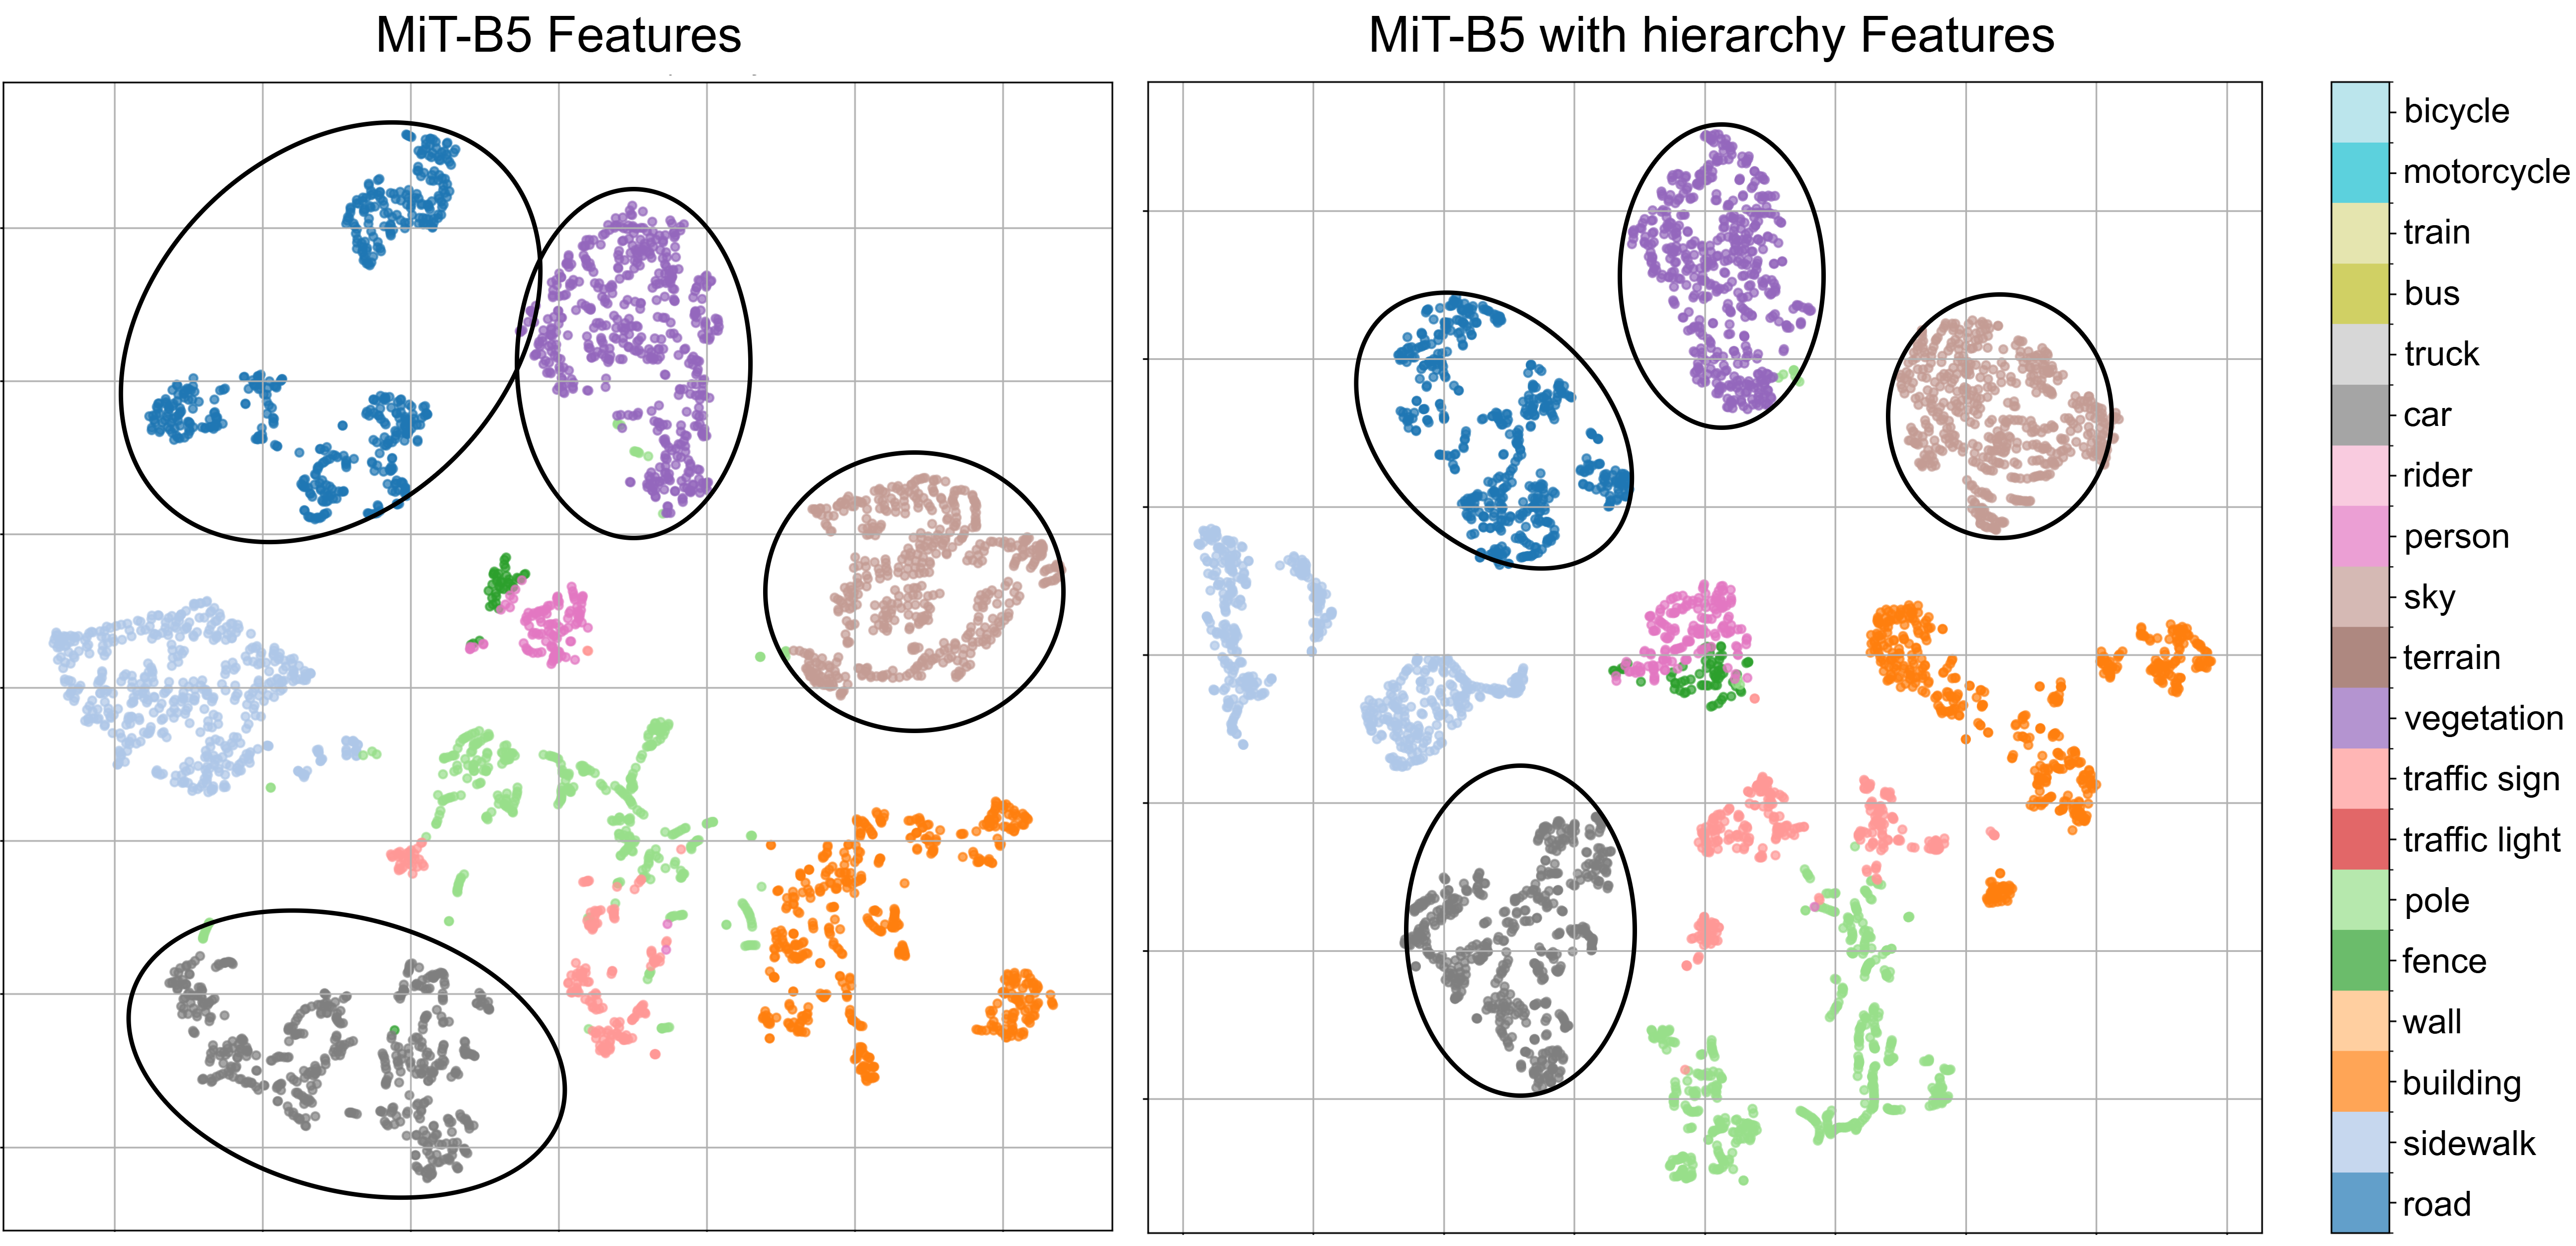
\includegraphics[width=0.5\textwidth]{figure3.png} % 插入图片
    \caption{T-SNE of features from MiT-B5 on the Cityscapes validation set. More compact and well-separated category clusters are formed for classes such as ``Road'', ``Vegetation'', ``Terrain'', and ``Car'', indicating enhanced discriminative capability and better alignment with the semantic hierarchical structure.} % 添加标题
    \label{fig:tsne} % 添加标签,用于文中引用
\end{figure}

It is evident from Figure~\ref{fig:tsne} that, after incorporating the hyperbolic hierarchical structure, the samples of the same class in the target domain become more tightly clustered, forming denser groups. This indicates that the learned features exhibit greater intra-class consistency in the high-dimensional space, with feature representations of samples from the same class being highly similar. This demonstrates that category-specific knowledge from the source domain is more completely and clearly generalized to the target domain, contributing to the separation of semantically similar categories. A possible explanation for this phenomenon is that, within the hyperbolic hierarchical structure, the explicit learning of abstract categories constrains the model’s learning of domain-generalization knowledge for a single category, encouraging it to acquire more common and useful knowledge from sibling classes while minimizing interference from other categories. This learning paradigm—grounded in the shared knowledge among multiple similar categories and focusing on their mutual differences—enables the model to better distinguish between similar classes.

To verify this, we calculated the cosine similarity between class prototypes on the target domain validation set, as shown in Figure~\ref{fig:cossim}. Darker colors indicate higher similarity, whereas lighter colors represent lower similarity. Our method yields a more structured and discriminative feature space, as evidenced by the clearer distinctions between dissimilar categories (lighter color blocks in non-diagonal regions) and much stronger similarity among semantically related categories (darker regions near the diagonal). These results demonstrate the effectiveness of our approach in learning superior semantic representations.
\begin{figure}[htbp]
    \centering

    % 第一行
    \begin{minipage}{0.34\textwidth}
        \centering
        \includegraphics[width=\linewidth]{figure4a.png}
        \\
        \small (a) Origin % 手动添加简单标注
    \end{minipage}
    \begin{minipage}{0.35\textwidth}
        \centering
        \includegraphics[width=\linewidth]{figure4b.png}
        \\
        \small (b) Ours % 手动添加简单标注
    \end{minipage}

    \caption{Comparison of class similarity matrices. This cosine similarity matrix visualizes the pairwise semantic relationships among different categories (such as ``Road'', ``Sidewalk'', and ``Building'') in the feature space. (a) shows the matrix generated by the baseline model, while (b) displays the matrix generated by our proposed method.}
    \label{fig:cossim}
\end{figure}

Although models inherently tend to produce highly similar features for samples from semantically similar classes, they may also exhibit high feature similarity for classes that are semantically quite different. For example, the classes ``Sidewalk'' and ``Terrain'' are not semantically related, yet a high cosine similarity of 0.79 is observed between them, likely due to factors such as their spatial proximity in images. After we introduce our method, the model's ability to learn domain-generalized knowledge across classes is constrained. As a result, the similarity between semantically similar classes remains largely unchanged, while the similarity between semantically dissimilar classes is generally reduced. In Figure~\ref{fig:cossim}, this phenomenon is reflected in the cosine similarity heatmap: the color intensity near the diagonal—which represents semantically similar categories—remains essentially stable, whereas the color intensity in other regions is noticeably diminished. This indicates that the model becomes less influenced by factors such as sample quantity or spatial adjacency that may otherwise cause high similarity between semantically unrelated classes, and instead focuses more on learning domain-generalized knowledge among semantically similar classes.

\textbf{Visualization}. In addition, we conduct qualitative analyses by visualizing our method's results on the target domain samples. As illustrated in Figure~\ref{fig:vis}, after integrating our approach, the model demonstrates improved performance in distinguishing category boundaries(Figure~\ref{fig:vis}, columns (c) and (d)). This enhancement is observed not only for common large-object categories such as ``Road'', but also for rare small-object categories such as ``Motorcycle'' and ``Rider''. The abstract hierarchical predictions(column (e) in Figure~\ref{fig:vis}) we present reveal that this improvement is evident as early as the model’s predictions of abstract categories, and subsequent predictions of specific categories represent further refinement and optimization(Figure~\ref{fig:vis}, column (d) and (e)). This directly highlights the role of progressive classification and explicit learning of abstract concepts in UDA tasks. Additionally, for certain categories absent from the ground truth, such as roadside signs($3^{rd}$ row in Figure~\ref{fig:vis}), their abstract concepts are analogous to ``Traffic Sign''. As a result, our method predicts them as the same category at the abstract hierarchical level($3^{rd}$ picture in column (e)). Although these objects are ultimately classified as ``Traffic Sign'', our method is more meaningful in upstream tasks compared to other methods that might ignore or randomly assign unknown objects.

\begin{figure}[htbp]
    \centering

    % 第一行
    \begin{minipage}{0.19\textwidth}
        \centering
        \includegraphics[width=\linewidth]{figure5a1.png}
    \end{minipage}
    \hfill
    \begin{minipage}{0.19\textwidth}
        \centering
        \includegraphics[width=\linewidth]{figure5b1.png}
    \end{minipage}
    \hfill
    \begin{minipage}{0.19\textwidth}
        \centering
        \includegraphics[width=\linewidth]{figure5c1.png}

    \end{minipage}
    \hfill
    \begin{minipage}{0.19\textwidth}
        \centering
        \includegraphics[width=\linewidth]{figure5d1.png}

    \end{minipage}
    \hfill
    \begin{minipage}{0.19\textwidth}
        \centering
        \includegraphics[width=\linewidth]{figure5e1.png}

    \end{minipage}

    % 行间垂直间距
    \vspace{0.2cm}

    % 第二行
    \begin{minipage}{0.19\textwidth}
        \centering
        \includegraphics[width=\linewidth]{figure5a2.png}

    \end{minipage}
    \hfill
    \begin{minipage}{0.19\textwidth}
        \centering
        \includegraphics[width=\linewidth]{figure5b2.png}

    \end{minipage}
    \hfill
    \begin{minipage}{0.19\textwidth}
        \centering
        \includegraphics[width=\linewidth]{figure5c2.png}

    \end{minipage}
    \hfill
    \begin{minipage}{0.19\textwidth}
        \centering
        \includegraphics[width=\linewidth]{figure5d2.png}

    \end{minipage}
    \hfill
    \begin{minipage}{0.19\textwidth}
        \centering
        \includegraphics[width=\linewidth]{figure5e2.png}

    \end{minipage}

    % 行间垂直间距
    \vspace{0.2cm}

    % 第三行
    \begin{minipage}[t]{0.19\textwidth}
        \centering
        \includegraphics[width=\linewidth]{figure5a3.png}
        \\ % 换行
        \small (a) Original Image % 手动添加简单标注
    \end{minipage}
    \hfill
    \begin{minipage}[t]{0.19\textwidth}
        \centering
        \includegraphics[width=\linewidth]{figure5b3.png}
        \\
        \small (b) Ground Truth \vphantom{g}
    \end{minipage}
    \hfill
    \begin{minipage}[t]{0.19\textwidth}
        \centering
        \includegraphics[width=\linewidth]{figure5c3.png}
        \\
        \small (c) Baseline \vphantom{g}
    \end{minipage}
    \hfill
    \begin{minipage}[t]{0.19\textwidth}
        \centering
        \includegraphics[width=\linewidth]{figure5d3.png}
        \\
        \small (d) Ours \vphantom{g}
    \end{minipage}
    \hfill
    \begin{minipage}[t]{0.19\textwidth}
        \centering
        \includegraphics[width=\linewidth]{figure5e3.png}
        \\
        \small (e) Hierarchy Pred. \vphantom{g}
    \end{minipage}

    \caption{Qualitative comparisons of different methods on GTA5 → Cityscapes. (c) denotes the predictions of the baseline model that uses the flat classification paradigm in Euclidean space. (d) denotes the predictions of the proposed model that performs progressive learning in hyperbolic space after incorporating explicit learning of abstract concepts for specific categories. (e) denotes the predictions of our model for abstract categories during the progressive learning process.}
    \label{fig:vis}
\end{figure}
\subsection{Ablation study}
\textbf{Selection of Hierarchical Structure.} Following the approach of \cite{atigh2022hyperbolic}, we artificially introduce hierarchical structures to induce inductive bias among predicted categories. However, since the rarity of different classes varies between the source and target domains, this scarcity may be further amplified through our proposed explicit learning of abstract knowledge based on hierarchical structures. The extent of this effect largely depends on the manually constructed hierarchy. In other words, an effective hierarchical structure should simultaneously account for the rationality of class induction and the balance of class scarcity. In practice, however, it is difficult to achieve both objectives. To investigate the impact of these two factors on UDA tasks, we designed two types of hierarchical structures: one prioritizing the rationality of class induction, and the other focusing on balancing class rarity, as shown in Figure~\ref{fig:hierarchys}. To explore which hierarchical structure is better suited to our method, we conducted experiments using both hierarchies. 

\begin{figure}[htbp]
    \centering

    % 第一行
    \begin{minipage}[t]{0.45\textwidth}
        \centering
        \includegraphics[height=5cm, keepaspectratio]{figure6a.png}
        \\
        \small (a) Reasonable structure $\mathcal{H}_{r}$ % 手动添加简单标注
        \label{fig:hie_reasonable}
    \end{minipage}
    \begin{minipage}[t]{0.45\textwidth}
        \centering
        \includegraphics[height=5cm, keepaspectratio]{figure6b.png}
        \\
        \small (b) Balanced structure $\mathcal{H}_{b}$% 手动添加简单标注
        \label{fig:hie_balanced}
    \end{minipage}

    \caption{Comparison of different hierarchical structures. (a) illustrates a hierarchy organized based on the inherent semantic relationships among categories, thus representing a structure that aligns with human cognitive logic. In contrast, (b) depicts a hierarchy organized based on category rarity, ensuring a relatively balanced sample size across categories at the same hierarchical depth. Since the abstract categories in this structure do not possess explicit semantic meaning, they are labeled as N1, N2, …, N9.}
    \label{fig:hierarchys}
\end{figure}


\begin{table}[h]
\centering
\tiny % 使用超小字体
\caption{Performance on Different Hierarchy Structure}
\label{tab:adp_hierarchy}
% 极度紧凑的布局
\setlength{\tabcolsep}{2pt} % 减少列间距
\renewcommand{\arraystretch}{1.1} % 减少行高

\begin{tabular}{@{}>{\centering\arraybackslash}m{3cm}| 
                >{\centering\arraybackslash}m{1.1cm}
                >{\centering\arraybackslash}m{1.1cm}|
                >{\centering\arraybackslash}m{1.1cm}
                >{\centering\arraybackslash}m{1.1cm}@{}}
\toprule
\textbf{\scriptsize Hierarchy} & \textbf{\scriptsize RCS} & 
\textbf{\scriptsize EL} & \textbf{\scriptsize mIoU} & \textbf{\scriptsize mAcc}\\
\midrule
\hyperref[fig:hie_reasonable]{$\mathcal{H}_{r}$} & - & - & 47.1 & 55.3 \\
\hyperref[fig:hie_reasonable]{$\mathcal{H}_{r}$} & \checkmark & - & 52.9 & 62.9 \\
\hyperref[fig:hie_reasonable]{$\mathcal{H}_{r}$} & \checkmark & \checkmark & 62.3 & 71.7 \\
\hyperref[fig:hie_reasonable]{$\mathcal{H}_{b}$} & - & - & 44.9 & 53.7 \\
\hyperref[fig:hie_reasonable]{$\mathcal{H}_{b}$} & \checkmark & - & 57.5 & 65.7 \\
\hyperref[fig:hie_reasonable]{$\mathcal{H}_{b}$} & \checkmark & \checkmark & 55.4 & 67.9 \\
\bottomrule
\end{tabular}
\end{table}

As shown in Table~\ref{tab:adp_hierarchy}, without the incorporation of the RCS strategy or explicit learning of abstract categories, a well-designed hierarchical structure enables the model to achieve superior performance in both mIoU and mAcc metrics. This indicates that the model exhibits enhanced knowledge generalization for both small and large objects. However, upon introducing the RCS strategy, improvements are observed in both metrics, with the balanced hierarchical structure experiencing a more pronounced enhancement. This demonstrates that the RCS strategy can simultaneously improve domain generalization of knowledge across different hierarchical structures, but its effect is more significant for structures that are already balanced. Moreover, the substantial improvement in mAcc indicates that even a balanced hierarchy remains highly sensitive to class imbalance. When we add explicit learning of abstract concepts, the balanced hierarchy’s mIoU can drop while its mAcc rises. This pattern suggests that under explicit abstract‑concept constraints the model reduces false positives (misclassifying other categories as the target) but at the cost of increased false negatives on marginal or ambiguous pixels of the target classes. By contrast, a semantically reasonable hierarchy yields large gains on both metrics. From these experiments we conclude that both the reasonableness of the hierarchical structure and the scarcity of classes can improve cross‑domain generalization, but the benefit of alleviating scarcity is most pronounced when the network has not yet learned reasonable inductive relationships among classes. Conversely, when class inductive validity is established, a well‑constructed hierarchy dominates and its benefits exceed those from addressing scarcity. Finally, explicit learning of abstract concepts only helps when the hierarchy encodes clear and semantically coherent relations among classes; otherwise it may degrade overall performance.

When explicit learning of abstract concepts is further incorporated, the performance of the balanced structure declines, whereas the reasonable hierarchical structure shows substantial improvement. Based on these experiments, we conclude that both the rationality of the hierarchical structure and the rarity of sample categories can enhance domain generalization of knowledge. The role of RCS is more prominent when the network lacks sufficient validation of reasonable category induction; conversely, when category induction is reasonable, it becomes the dominant factor, and a well-designed hierarchical structure offers greater advantages. Furthermore, the improvement brought by rationality surpasses that contributed by rarity.

\textbf{Manifold Space.} In conventional Euclidean space, models can learn some shared abstract concepts among categories through training. However, we argue that this learning capacity is inherently limited, as Euclidean space possesses restricted capability for perceiving hierarchical relationships between categories. While actively organizing hierarchical structures among categories and employing progressive learning paradigms can enhance a model’s ability to learn abstract concepts, such improvements fundamentally depend on the model’s capacity for hierarchical embedding within its underlying manifold space. To substantiate this point, we conduct UDA tasks with models operating in both Euclidean and Hyperbolic spaces, integrating our proposed method into each setting.

\begin{table}[h]
\centering
\tiny % 使用超小字体
\caption{Performance on Different Manifold Space}
\label{tab:adp_manifold}

% 极度紧凑的布局
\setlength{\tabcolsep}{2pt} % 减少列间距
\renewcommand{\arraystretch}{1.1} % 减少行高

\begin{tabular}{@{}>{\centering\arraybackslash}m{2.5cm}| 
                >{\centering\arraybackslash}m{2.5cm}|
                >{\centering\arraybackslash}m{1.1cm}
                >{\centering\arraybackslash}m{1.1cm}@{}}
\toprule
\textbf{\scriptsize Manifold Space} & \textbf{\scriptsize Hyper-HierUDA} & 
 \textbf{\scriptsize mIoU} & \textbf{\scriptsize mAcc}\\
\midrule
Euclidean & - & 65.07 & 75.9 \\
Euclidean & \checkmark & 60.3 & 70.3 \\
Hyperbolic & - & 55.4 & 64.8 \\
Hyperbolic & \checkmark & 70.05 & 80.24 \\
\bottomrule
\end{tabular}
\end{table}

As shown in Table~\ref{tab:adp_manifold}, due to the limited hierarchical embedding capacity of Euclidean space, our method actually leads to a slight decrease in model performance. Furthermore, in hyperbolic space without explicit hierarchical constraints, the model's performance in hyperbolic space is substantially inferior to that in Euclidean space. This observation is consistent with conclusions drawn in \cite{halo2021hyperbolic}. However, when hierarchical structures are actively introduced—surpassing the conventional metric learning paradigm—our method enables the model to exceed its previous performance in Euclidean space.

\textbf{Curvature in Hyperbolic Space.} In the Poincaré model of hyperbolic space, the curvature parameter $\mathit{c}$ is a critical hyperparameter that governs both the curvature and the radius of the Poincaré ball. The value of $\mathit{c}$ determines the degree of boundary distortion in the Poincaré ball. One key advantage of hyperbolic space is its ability to embed hierarchical structures with minimal distortion, and the compactness of such embeddings is dictated by the curvature $\mathit{c}$. Given that UDA tasks typically involve a relatively small number of categories and simple hierarchical structures, we posit that a lower curvature is more suitable in this context. To validate this hypothesis, we conducted experiments with different curvature values.

As illustrated in Table~\ref{tab:adp_c}, the highest mIoU of 70.0 is achieved at a curvature of 0.5, indicating an optimal embedding compactness for this specific task. In contrast, both lower and higher curvature values result in comparatively reduced performance: mIoU values are 64.0, 64.4, 63.0, and 65.0 for curvatures of 0.1, 0.25, 0.75, and 1.0, respectively. These results support the initial hypothesis that a relatively low curvature is more suitable for UDA, likely due to its simpler hierarchical structure and limited number of classes. The superior performance at $\mathit{c}$=0.5 suggests that an appropriately chosen curvature can enhance structural representation with minimal distortion, thereby improving segmentation accuracy. This experiment underscores the importance of curvature selection in hyperbolic neural architectures for UDA tasks.

\begin{table}
\centering
\tiny % 使用超小字体
\caption{Performance with Different Curvature}
\label{tab:adp_c}

% 极度紧凑的布局
\setlength{\tabcolsep}{2pt} % 减少列间距
\renewcommand{\arraystretch}{1.1} % 减少行高

\begin{tabular}{@{}>{\centering\arraybackslash}p{1.1cm}| 
                *{5}{>{\centering\arraybackslash}p{1.1cm}}
}
\toprule

c & 0.1 & 0.25 & 0.5 & 0.75 & 1.0 \\
\midrule
mIoU & 64.0 & 64.4 & 70.0 & 63.0 & 65.0 \\

\bottomrule
\end{tabular}
\end{table}


\section{Conclusions}
In this paper, we propose Hyper-HierUDA and systematically explore the integration of hyperbolic geometry into UDA for semantic segmentation, thus moving beyond the conventional flat classification paradigm. Our investigation confirms that explicitly modeling and learning the inherent semantic hierarchy among categories can significantly enhance the model's ability to generalize knowledge across domains. The core of our approach lies in a novel progressive classification framework in the hyperbolic space, which is complemented by an explicit learning strategy for abstract concepts.

\textbf{Limitations.} Our method still has several limitations. First, following prior work, we adopt the Poincaré model for modeling and embedding in hyperbolic space. However, the Poincaré model itself is prone to training instability, with issues such as gradient explosion frequently occurring in practice. Moreover, its nonlinear operations (such as Möbius addition) are computationally complex, requiring more training resources and higher costs. 
In addition, although we have demonstrated the architectural generalizability of our method in UDA tasks, its effectiveness in certain upstream tasks (e.g., domain adaptation, DA) is limited. Specifically, our approach is only effective on Transformer-based models, while performance on CNN-based models is suboptimal. Therefore, further exploration and optimization are required to extend our method to these upstream tasks.
At last, although our method is grounded in hyperbolic neural networks, the instantiation we use is an end‑to‑end hybrid model. The bulk of computations is carried out in Euclidean space, and Euclidean features are mapped into hyperbolic space only at the final layer to obtain hierarchical representations. In contrast, a true hyperbolic neural network performs the entire computation—from input to output—within hyperbolic space, thereby preserving the manifold’s geometric properties to a greater extent. Adapting our method to a true hyperbolic architecture would therefore necessitate designing a corresponding network from scratch.

%% The Appendices part is started with the command \appendix;
%% appendix sections are then done as normal sections


%% For citations use: 
%%       \cite{<label>} ==> [1]


% 或者使用 \acknowledgments 或 \acknowledgement,具体看模板要求

%%
% Example citation, See \cite{lamport94}.

%% If you have bib database file and want bibtex to generate the
%% bibitems, please use
%%
\bibliographystyle{elsarticle-num} 
\bibliography{reference.bib}

%% else use the following coding to input the bibitems directly in the
%% TeX file.

%% Refer following link for more details about bibliography and citations.
%% https://en.wikibooks.org/wiki/LaTeX/Bibliography_Management

% \begin{thebibliography}{00}

% %% For numbered reference style
% %% \bibitem{label}
% %% Text of bibliographic item

% \bibitem{lamport94}
%   Leslie Lamport,
%   \textit{\LaTeX: a document preparation system},
%   Addison Wesley, Massachusetts,
%   2nd edition,
%   1994.

% \end{thebibliography}
\end{document}

\endinput
%%
%% End of file `elsarticle-template-num.tex'.
